% !TEX TS-program = xelatex

\documentclass{resume}

\usepackage{fancyhdr}
\usepackage{datetime}

% 定义更新日期
\newdateformat{chinesedate}{\THEYEAR 年 \twodigit{\THEMONTH} 月 \twodigit{\THEDAY} 日}
\newdate{lastupdated}{\day}{\month}{\year}

% \usepackage[margin=1in, headsep=2cm, footskip=2cm]{geometry}

% 设置页眉样式
\fancypagestyle{myheader}{%
  \fancyhf{}% 清空页眉页脚
  \renewcommand{\headrulewidth}{0pt}% 移除页眉线
  \fancyfootoffset[R]{1cm}% 设置右边页脚的偏移量
  \fancyfoot[R]{更新日期: \chinesedate\displaydate{lastupdated}}% 在右上角添加更新日期
}
\pagestyle{myheader}% 应用定义的页眉样式

\usepackage{zh_CN-Adobefonts_external} % Simplified Chinese Support using external fonts (./fonts/zh_CN-Adobe/)
%\usepackage{zh_CN-Adobefonts_internal} % Simplified Chinese Support using system fonts
\usepackage{linespacing_fix} % disable extra space before next section
\usepackage{cite}
\usepackage{multirow}
\usepackage{graphicx}
\usepackage{tabu}

\begin{document}
\pagenumbering{gobble} % suppress displaying page number

\Large{
  \begin{tabu}{ p{0.3\textwidth} p{0.7\textwidth} }
   \multirow{4}{2in}{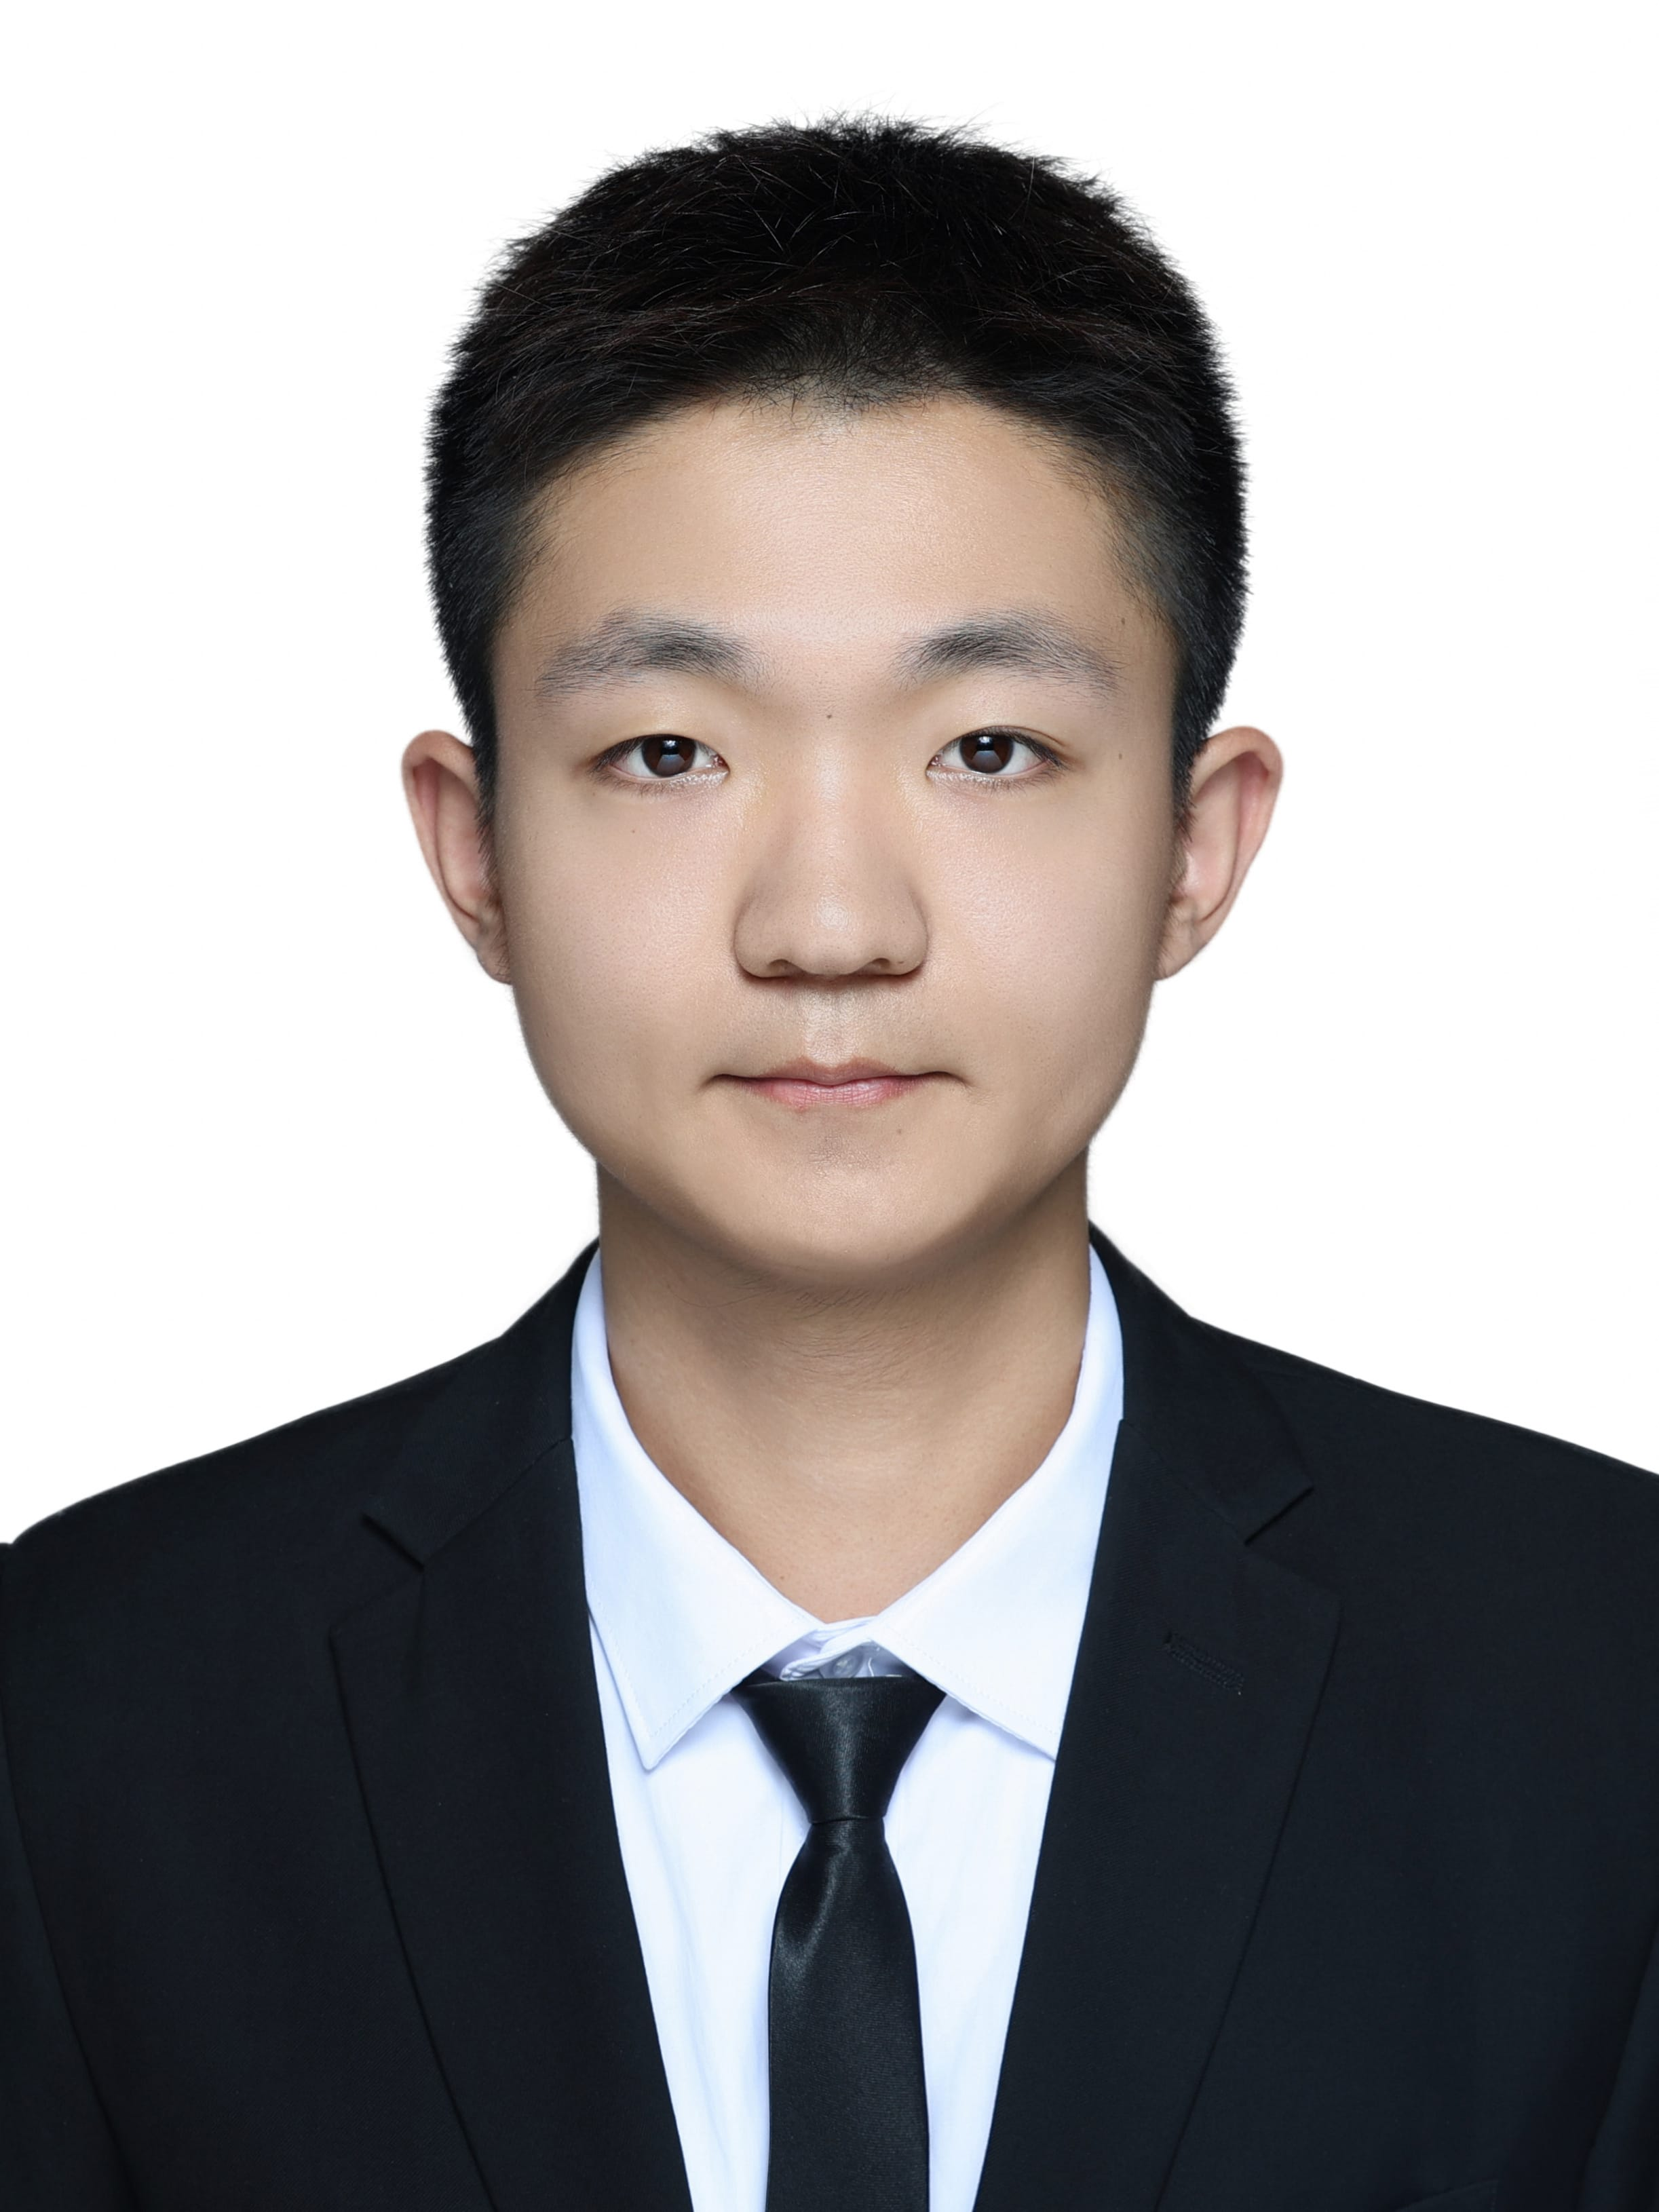
\includegraphics[width=1.2in]{resume/p1.jpg}}
    & \raggedright \textbf{\fontsize{20}{24}\selectfont{林德松}}  \\
    \\
    & \scshape{Lin Desong} \textperiodcentered \\
    & \email{lindesong666@163.com}  \\
    & \phone{(+86) 187-6338-6500} \\
    & \github[gitee.com/desonglll]{https://gitee.com/desonglll} \\
  \end{tabu}
}

\hspace{}

\section{\faGraduationCap\  教育背景}

\datedsubsection{\textbf{曲阜师范大学}, 济宁, 山东}{2020 -- 2024}
\textit{学士学位}\ 软件工程

\section{\faUsers\ 实习/项目经历}

\datedsubsection{\textbf{\href{https://gitee.com/desonglll/new-ez-stock}{EzStock管理系统}}}{2023年12月 -- 至今}
\role{Python, Django, React, TypeScript——个人开源项目}

\datedsubsection{\textbf{江苏传智播客教育科技股份有限公司济南分公司}, 济南}{2023年12月 -- 2024年2月}
\role{SpringBoot MVC后端开发} % {指导老师: 邹风蒙}

\datedsubsection{\textbf{e和园校园服务管理平台}}{2022年3月 -- 2022年9月}
\role{微信小程序——团队项目}

\datedsubsection{\textbf{济续游宁}}{2022年3月 -- 2022年9月}
\role{微信小程序——团队项目}

\datedsubsection{\textbf{党团助手一校园党建平台}}{2022年3月 -- 2022年8月}
\role{微信小程序——团队项目}

\section{\faCogs\ IT 技能}
% increase linespacing [parsep=0.5ex]
\begin{itemize}[label=$\bullet$, parsep=0.5ex]
  \item 编程语言: Python == Java > Rust == C++
  \begin{itemize}[leftmargin=*, itemsep=5pt]
      \item 系统级编程语言: Rust 、 C++ 、 C 、 GoLang
      \item 高级编程语言: Python 、 Java 
      \item 应用级编程语言: Swift 、 Swift UI
      \item 脚本语言: Lua 、 TypeScript 、 JavaScript
      \item 数值分析语言: Julia
  \end{itemize}
  \item 平台: macOS, Linux
  \item 开发: 
  \begin{itemize}
      \item 熟练使用Anaconda、Jupyter Notebook、Nginx 、 Docker等工具
      \item 熟练掌握使用Vim、Tmux、Git等开发工具
      \item 熟练掌握Linux命令、SSH远程通信
  \end{itemize}
  \item 技能: 
      \begin{itemize}
      \item 熟练掌握Python常见的Web框架:
        \begin{itemize}
      \item Django, Django Rest-Framework
      \item Flask
      \item FastAPI
  \end{itemize}
      \item 熟练掌握Java常见的Web框架:
        \begin{itemize}
            \item Spring、 SpringBoot
            \item SpringMVC、MyBatis
        \end{itemize}
      \item 熟练使用 MySQL 关系型数据库
      \item 熟练使用 Redis、 MongoDB 非关系型数据库
      \item 掌握项目的构建与依赖管理工具 Maven、Gradle
      % \item 熟练使用 SpringCloud 微服务架构及相关组件的运用,并拥有实际的微服务项目开发经验
      \item 熟悉常见的 Web 服务器,Tomcat,对 HTTP 协议有深入的了解,熟练掌握 Rest 风格接口开发
      \item 熟悉前端框架开发,对 React TS, AntDesign, MaterialUI 熟练开发
      % \item 熟悉 Spring 中的 IOC 和 AOP 的思想
      \item 数据采集与整理:使用爬虫技术抓取数据,进行数据分析
      \begin{itemize}
          \item Scrapy框架
          \item Julia数据分析
      \end{itemize}
  \end{itemize}

\end{itemize}

\section{\faHeartO\ 获奖/证书情况}
\datedline{\textit{校三等奖学金}, 曲阜师范大学“三等奖学金”}{2021 年10 月}
\datedline{\textit{省二等奖}, 第十九届山东省大学生软件设计大赛}{2021 年11 月}
\datedline{\textit{校二等奖学金}, 曲阜师范大学“二等奖学金”}{2022 年10 月}
\datedline{\textit{优秀团员}, 曲阜师范大学“优秀团员”}{2022 年10 月}
\datedline{\textit{省二等奖}, 第二十届山东省大学生软件设计大赛——党团助手}{2022 年10 月}
\datedline{\textit{省三等奖}, 第二十届山东省大学生软件设计大赛——济续游宁}{2022 年10 月}
\datedline{\textit{软件著作权}, 党团助手——校园党建平台}{2023 年01 月}
\datedline{\textit{软件著作权}, e和园校园服务管理平台}{2023 年02 月}
\datedline{\textit{省一等奖}, 第十五届全国大学生数学竞赛山东赛区}{2023 年11 月}
\datedline{\textit{校三等奖学金}, 曲阜师范大学“三等奖学金”}{2023 年11 月}
\datedline{\textit{山东省优秀毕业生}, 2024届山东省优秀毕业生}{2024 年01 月}
\section{\faInfo\ 其他}
% increase linespacing [parsep=0.5ex]
\begin{itemize}[parsep=0.5ex]
  \item Gitee: https://gitee.com/desonglll
  \item 语言: 英语 - 熟练(英语六级)
\end{itemize}

%% Reference
%\newpage
%\bibliographystyle{IEEETran}
%\bibliography{mycite}
\end{document}
